Hogy információt szerezzek arról, hogyan viselkedik az alkalmazás nagyobb terhelés esetén, és hogy megvizsgáljam a rendszerrel szemben állított nem funkcionális igények  (\ref{sec:indikatorok}~pont)  teljesülését,	terheléses teljesítményvizsgálatnak vetettem alá a létrehozott helpdesk programot.


\section{Terheléses teszt}
A terheléses teszt egy --a teljesítménytesztelés alá tartozó-- nem funkcionális vizsgálat. Célja a rendszer működésének vizsgálata, viselkedésének megértése bizonyos előre meghatározott terhelés esetén.

A vizsgálat párhuzamos felhasználók modellezésén alapszik. A vizsgált alkalmazás folyamatos monitorozás alatt áll, miközben a felhasználók --azonos időben-- végre próbálják hajtani az előre meghatározott üzleti igényeiket.

A tesztelés során rögzített válaszidőket ezután célszerű összevetni a rendszer metrikáival, hogy feltárhatóak legyenek az alkalmazás összteljesítményét kritikusan érintő szűk keresztmetszetek.


\section{Apache JMeter}	
Az Apache Jmeter egy nyílt forrású terheléses teszt végrehajtására alkalmas eszköz. Számos protokollt képes kezelni, a helpdesk alkalmazás vizsgálatánál HTTP üzenetek küldésével modelleztem a párhuzamos felhasználókat.

Mivel a helpdesk frontend a kliens oldalon (\ref{sec:angular}~pont) --a felhasználó számítógépén-- fut, így elegendő csak a frontend-backend közötti kommunikációt imitálni.

Minden teszt egy rövid felfutási idővel kezdődik, ami során a JMeter elindítja a párhuzamos teszteléshez használt szálakat (\ref{fig:active_threads_over_time} ábra). A szálak --a teszt teljes ideje alatt-- folyamatosan hajtják végre a számukra kijelölt feladatot. A JMeter méri és rögzíti a vizsgált rendszer válaszait és válaszidejét. A rögzített adatok további elemzésével meghatározható a vizsgált rendszer viselkedése, a Grafana-ban megjelenített metrikák összevetésével pedig azonosíthatóak a teljesítmény szempontjából kritikus rendszerek.

A létrehozott JMeter tesztjeim a leggyakrabban és a legtöbb erőforrást igénylő funkciókat tesztelik $120$~másodpercig.


\begin{figure}[hbt] 
	\centering
	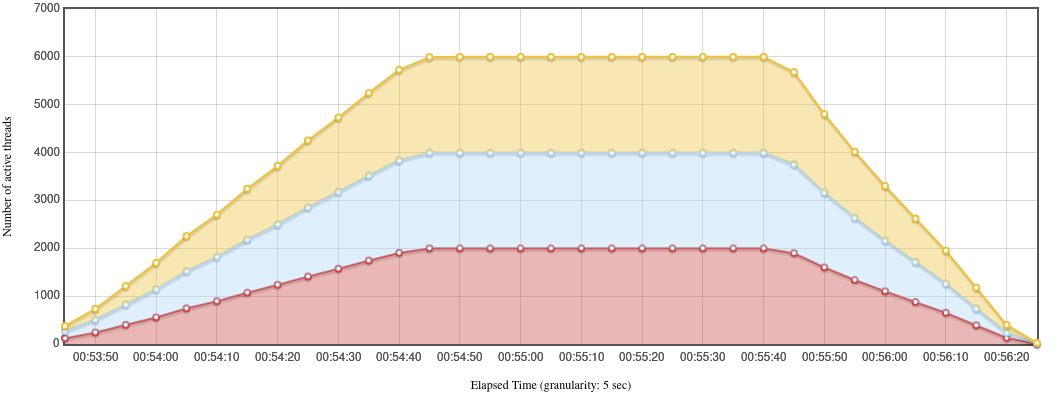
\includegraphics[width=0.8\textwidth]{active_threads_over_time.png}
	\caption[A JMeter tesztelés során használt-- szálai]{A JMeter --tesztelés során használt-- szálai. A különböző üzleti funkciókat hívó szálak eltérő színnel szerepelnek.}
	\label{fig:active_threads_over_time}
	\floatfoot{Forrás: saját ábra}
\end{figure}



\section{Átlagos teljesítmény vizsgálata}
A helpdesk backend egy önálló példányát vizsgáltam $100$ párhuzamos felhasználó modellezésével. A teszt során használt felfutási idő $30$~másodperc volt.

A teszt eredményeit \aref{tabl:1_instance_100_user} táblázat tartalmazza.

\begin{table}[hbt]
	
	\begin{tabular}{ccccc|c|cc}
		\multicolumn{5}{c|}{Válaszidő [$ms$]}  & Áteresztőképesség & \multicolumn{2}{c}{Válasz [\%]}	\\
		Átlag & Max. & Medián & P90 & P95 &	[Tranzakció$/s$] & $<3s$& $<6s$ \\
		\hline 
		99,32 & 856 & 88,00 & 223,00 & 340,00 & 900,01 & 100 & 100 \\
	\end{tabular} 
	
	\caption{Egy példányban futó helpdesk backend terheléses teszt eredménye $100$ felhasználóval}
	\label{tabl:1_instance_100_user}
\end{table}

\Aref{fig:1_instance_100_user} ábrán és \aref{tabl:1_instance_100_user} táblázat adataiból látszódik, hogy:
\begin{itemize}
	\item a legtöbb válasz 88~$ms$ alatt megérkezik,
	\item a backend legrosszabb esetben is 1 másodperc alatt válaszol,
	\item a rendszer áteresztőképessége 900 tranzakció másodpercenként.
\end{itemize}


\begin{figure}[hbt]
	\begin{subfigure}{.9\textwidth}
		\centering
		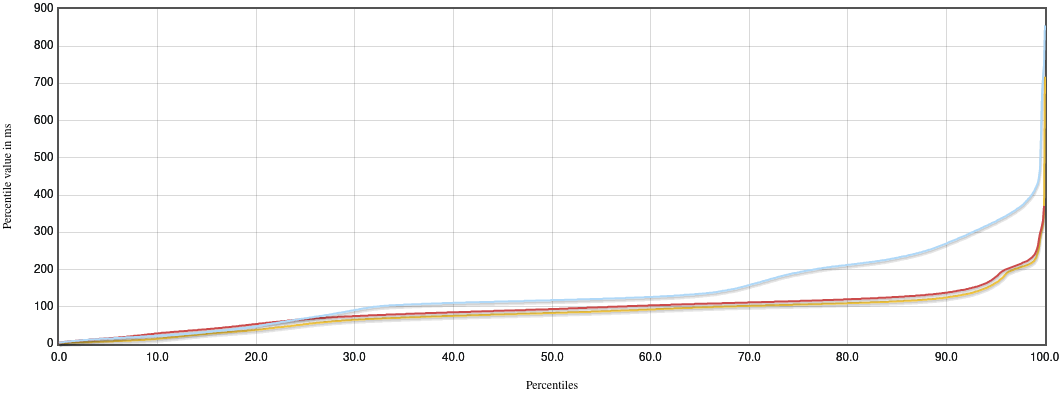
\includegraphics[width=.9\linewidth]{100_user_flotResponseTimesPercentiles.png}  
		\caption{A válaszidők percentilis eloszlása}
	\end{subfigure}
	\begin{subfigure}{.9\textwidth}
		\centering
		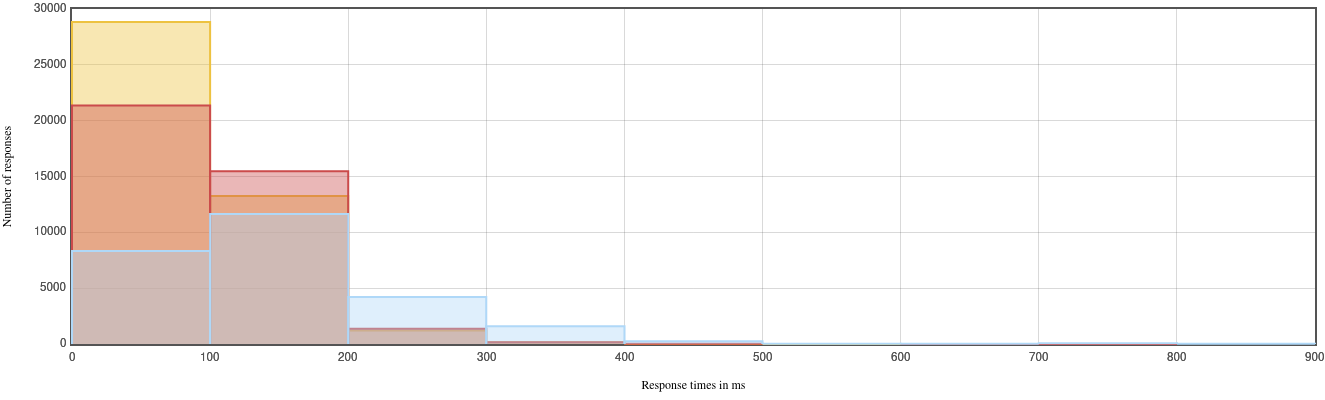
\includegraphics[width=.9\linewidth]{100_user_flotResponseTimeDistribution.png}  
		\caption{A válaszidők eloszlása}
	\end{subfigure}
	
	\caption[Helpdesk backend terheléses teszt 100 felhasználóval]{Egy példányban futó helpdesk backend terheléses teszt eredménye $100$ felhasználóval}
	\floatfoot{Forrás: saját ábra}
	\label{fig:1_instance_100_user}
\end{figure}

Az alkalmazás tehát megfelel a vele szemben állított követelményeknek.



\section{Csúcsteljesítmény vizsgálata}\label{sec:peak_1_instance}
A helpdesk backend egy önálló példányát vizsgáltam $6~000$ párhuzamos felhasználó modellezésével. Mint ahogy a teszt során használt párhuzamos szálakról készített \aref{fig:active_threads_over_time} ábrán is látszódik, a felfutási idő $60$~másodperc volt. Az ábrán látható ahogy a JMeter a felfutási idő után egyszerre $6~000$ szálon futtatja a teszteket.

A teszt futtatása során mért eredményeket \aref{tabl:1_instance_10_hikkari_nginx} táblázatban foglaltam össze. Mint láthatjuk, az alkalmazás messze elmarad a vele szemben állított követelményektől (\ref{sec:indikatorok}~pont). Három másodperc alatt csak a kérések $10,19\%$-át szolgálja ki. A legtöbb kérésre 25~másodpercet vesz igénybe a válasz adása.

\begin{table}[hbt]

		\begin{tabular}{ccccc|c|cc}
			\multicolumn{5}{c|}{Válaszidő [$ms$]}  & Áteresztőképesség & \multicolumn{2}{c}{Válasz [\%]}	\\
			Átlag & Max. & Medián & P90 & P95 &	[Tranzakció$/s$] & $<3s$& $<6s$ \\
			\hline 
			15 133,81 & 31 732 & 24 553,00 & 28 011 & 28 407  & 281,72 &	10,19 & 27,78 \\
		\end{tabular} 

	\caption{Egy példányban futó helpdesk backend terheléses teszt eredménye $6~000$ felhasználóval}
	\label{tabl:1_instance_10_hikkari_nginx}
\end{table}

Az eltérés okainak azonosítására célszerű a szűk keresztmetszeteket meghatározni és feloldani~(\ref{sec:bottleneck} pont).

\begin{figure}[hbt]
	\begin{subfigure}{.9\textwidth}
		\centering
		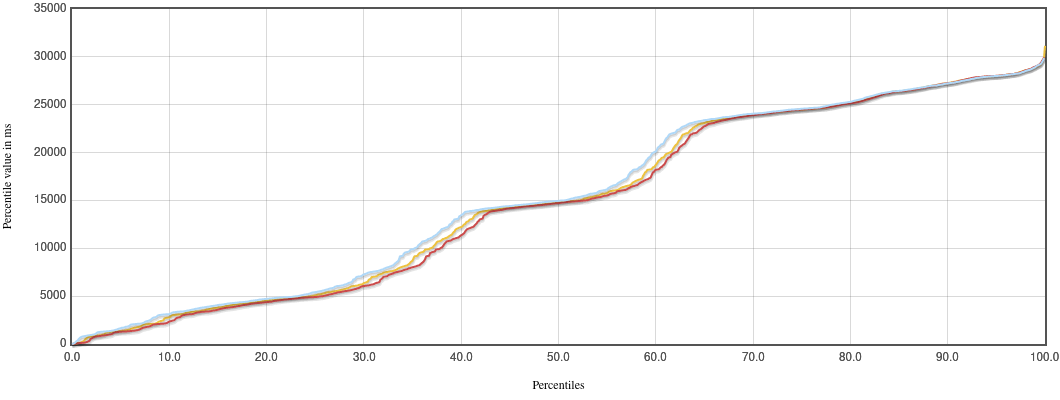
\includegraphics[width=.9\linewidth]{1instance_10_hikkari_nginx_flotResponseTimesPercentiles.png}  
		\caption{A válaszidők percentilis eloszlása}
	\end{subfigure}
	\begin{subfigure}{.9\textwidth}
		\centering
		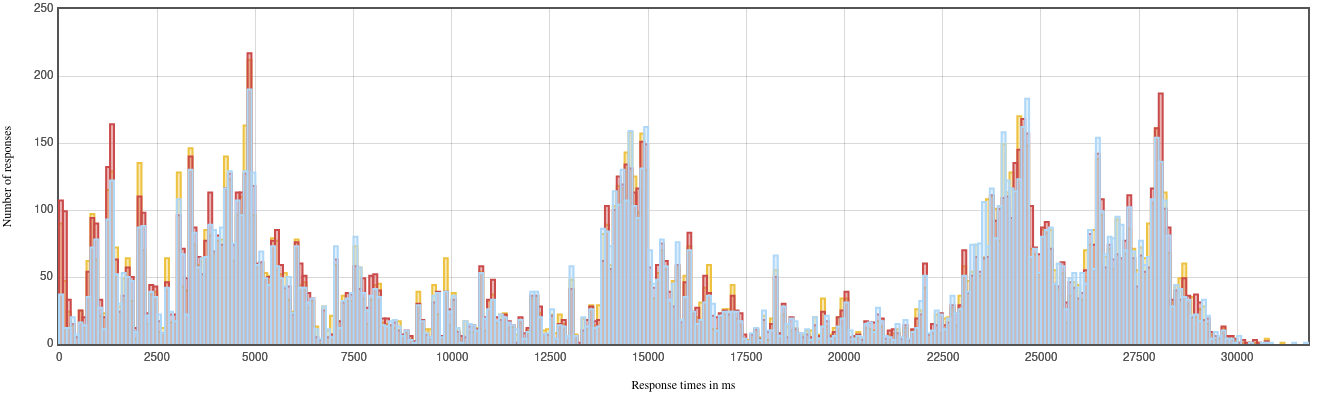
\includegraphics[width=.9\linewidth]{1instance_10_hikkari_nginx_flotResponseTimeDistribution.png}  
		\caption{A válaszidők eloszlása}
	\end{subfigure}
	
	\caption[Helpdesk backend terheléses teszt egy példánnyal]{Egy példányban futó helpdesk backend terheléses teszt eredménye $6~000$ felhasználóval}
	\floatfoot{Forrás: saját ábra}
\end{figure}

\pagebreak

\section{Szűk keresztmetszet meghatározása}\label{sec:bottleneck}
A JMeter által indított kérés az alábbi rendszereken megy keresztül (\ref{fig:jmeter_sequence}~ábra):
\begin{enumerate}
	\item Az Nginx fogadja és továbbítja a HTTP kérést a Helpdesk backendnek.
	\item A backend végrehajtja az üzleti funkciót, és amennyiben szükséges
	\item lekérdezi és visszaadja az eltárolt adatokat az adatbázisból. 
\end{enumerate}

\begin{figure}[hbt] 
	\centering
	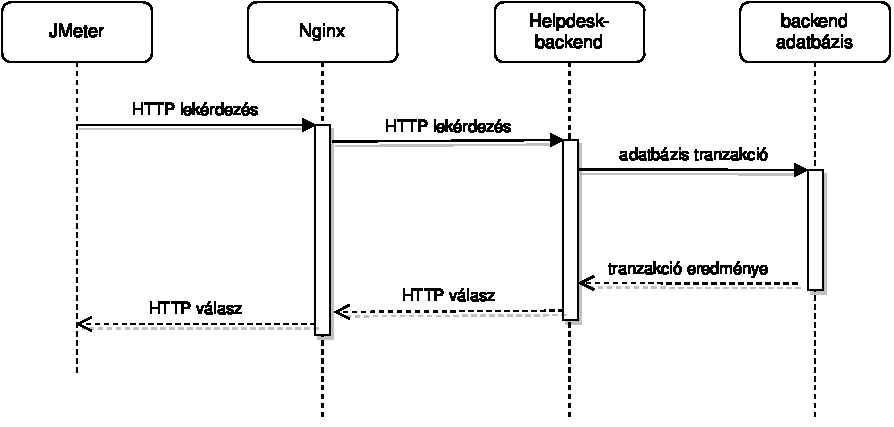
\includegraphics[width=0.8\textwidth]{jmeter_sequence_diagram_drawio.pdf}
	\caption{A terheléses tesztben résztvevő alkalmazások}
	\label{fig:jmeter_sequence}
	\floatfoot{Forrás: saját ábra}
\end{figure}



Így a szűk keresztmetszet is csak ebben a három rendszerben fordulhat elő. A backend metrikáinak vizsgálatából látszódik, hogy:
\begin{itemize}
	\item A backend memóriaigénye nem nőtt meg jelentősen (\ref{fig:memory_1_instance}~ábra).
	
	\item A processzorigény szignifikánsan megemelkedett (\ref{fig:cpu_1_instance}~ábra). A rendszer CPU felhasználása 80\%-ra a backendé 40\%ra nőtt.
	
	\item Az adatbázis kapcsolatok fenntartására használt HikariCP-ben (\ref{sec:adatbazis} pont) lényegesen feltorlódtak a lekérdezések (\ref{fig:10_hikari}~ábra). A függőben lévő kapcsolatok markánsan megugrottak.
\end{itemize}


\begin{figure}[hbt]
	\begin{subfigure}{.95\textwidth}
		\centering
		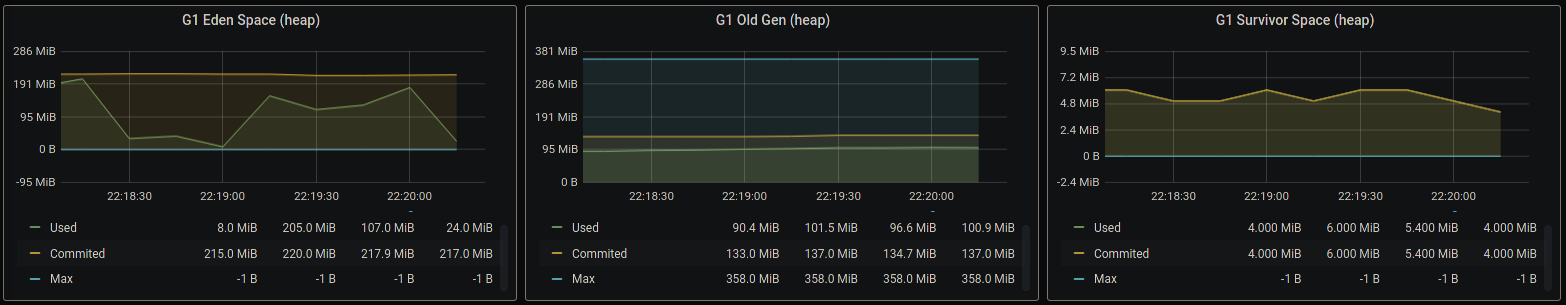
\includegraphics[width=.95\linewidth]{Memory_1_instance.png}  
		\caption{A backend memóriafelhasználása}
		\label{fig:memory_1_instance}

	\end{subfigure}
	\quad

	\begin{subfigure}{.6\textwidth}
		\centering
		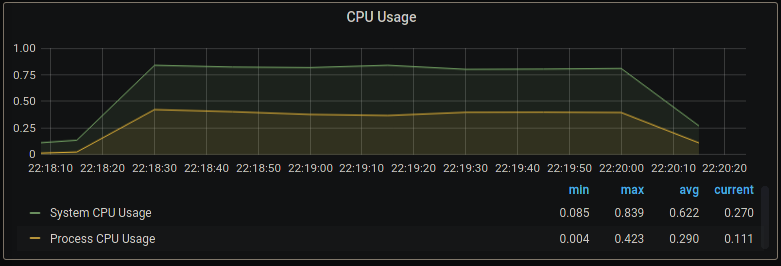
\includegraphics[width=.9\linewidth]{CPU_1_instance.png}  
		\caption{A backend processzor használata}
		\label{fig:cpu_1_instance}
	\end{subfigure}

	\quad
	\begin{subfigure}{.8\textwidth}
		\centering
		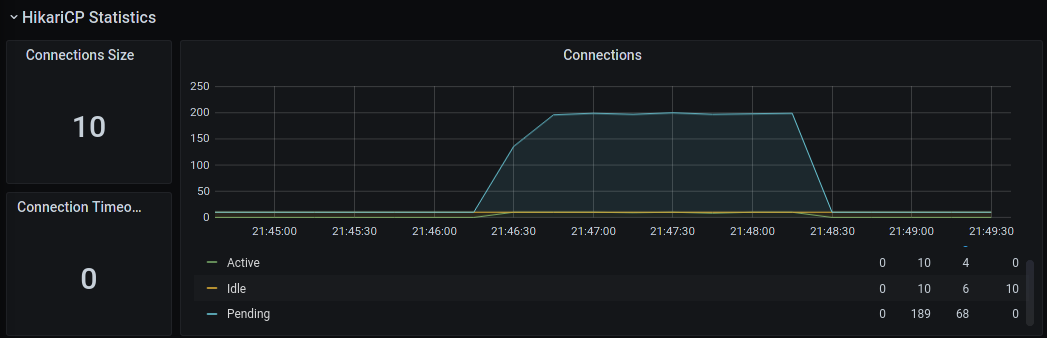
\includegraphics[width=.9\linewidth]{hikari_10.png}  
		\caption{HikariCP adatbázis-kapcsolatai}
		\label{fig:10_hikari}
	\end{subfigure}
	
	\caption{A csúcsteljesítmény vizsgálata során vizsgált legfontosabb metrikák}
	\label{fig:peak_metrics}
	\floatfoot{Forrás: saját ábra}
\end{figure}

\pagebreak

\subsection{Nginx}
Hogy az Nginx párhuzamosan kiszolgáljon legalább $6~000$ felhasználót\footnote{Az alapbeállítás $1~024$ kapcsolat}, a beállításaiban felül kell írni a \mbox{\textit{worker\textunderscore connections}} paramétert.

Ha az alapbeállításoktól való eltérés okozza a kérések --még backend előtti-- feltorlódását, vagy a megnövekedett processzorigényt, akkor az Nginx kihagyásával jelentős javulás lenne elérhető.

\bigskip
\begin{table}[hbt]
	
	\begin{tabular}{ccccc|c|cc}
		\multicolumn{5}{c|}{Válaszidő [$ms$]}  & Áteresztőképesség & \multicolumn{2}{c}{Válasz [\%]}	\\
		Átlag & Max. & Medián & P90 & P95 &	[Tranzakció$/s$] & $<3s$& $<6s$ \\
		\hline 
		15 772,71 &  49 367 & 29 450,00 & 34 256 & 34 898 & 265,72 & 26,41 & 36,78 \\
	\end{tabular} 
	
	\caption{Nginx nélkül futó helpdesk backend terheléses teszt eredménye $6~000$ felhasználóval}
	\label{tabl:without_nginx}
\end{table}

Ezért a megismételt a JMeter tesztben a backendet közvetlenül az IP-címén keresztül értem el. Az új mérés --\ref{tabl:without_nginx} táblázat-- adataiból látszódik, hogy

\begin{itemize}
	\item az átlagos és a medián válaszidő, valamint áteresztőképesség nem változott,
	\item a három másodperc alatt megérkező válaszok aránya --az első esethez (\ref{sec:peak_1_instance}) képest-- meg két és félszereződött, $26,41\%$-ra nőtt.
\end{itemize}



Ugyanez jelenik meg \aref{fig:without_nginx_min_median_max_over_time} ábrán is, a teszt első háromnegyedében a backend néhány kérésre azonnal válaszol, míg a többségre --medián-- csak sokkal később.

\begin{figure}[hbt]
	\begin{subfigure}{.49\textwidth}
		\centering
		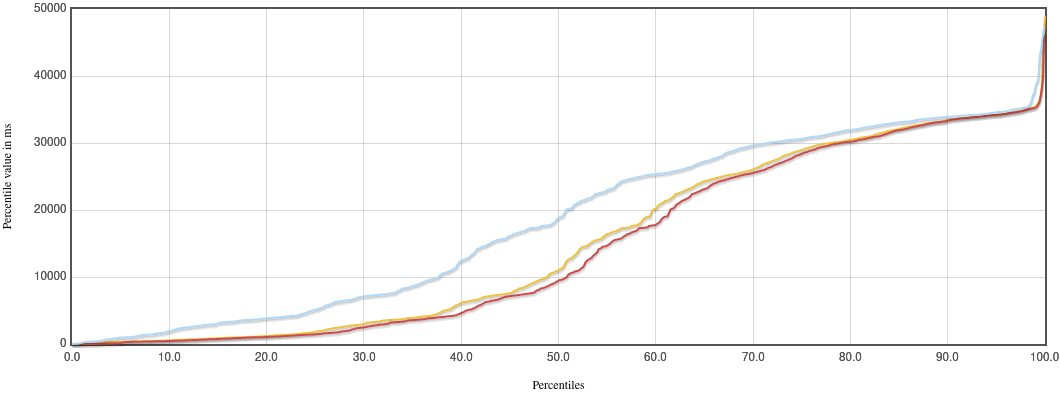
\includegraphics[width=.9\linewidth]{without_nginx_flotResponseTimesPercentiles.png}  
		\caption{A válaszidők percentilis eloszlása}
		\label{fig:without_nginx_percentil}
	\end{subfigure}
	\begin{subfigure}{.49\textwidth}
		\centering
		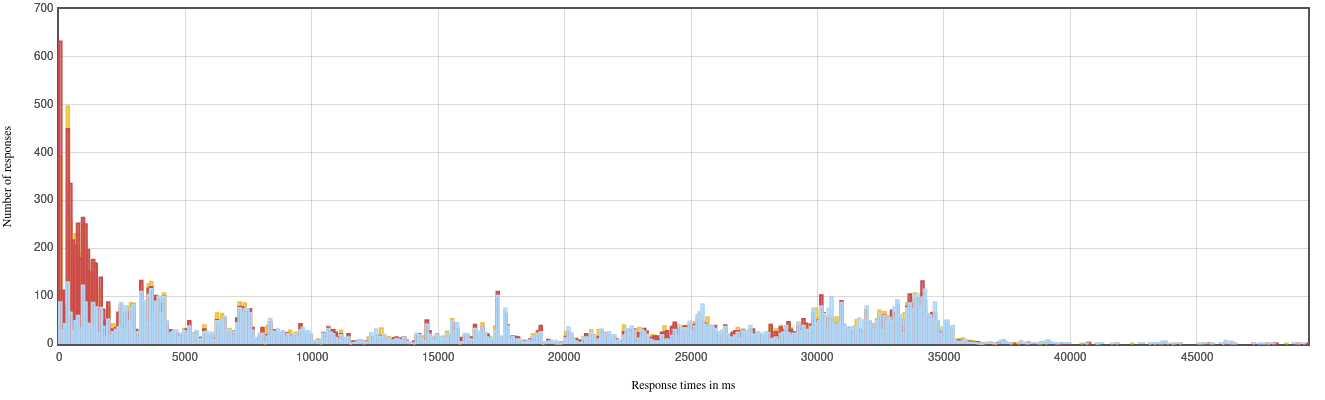
\includegraphics[width=.9\linewidth]{without_nginx_flotResponseTimeDistribution.png}  
		\caption{A válaszidők eloszlása}
	\end{subfigure}
	
	\quad
	
	\begin{subfigure}{.95\textwidth}
		\centering
		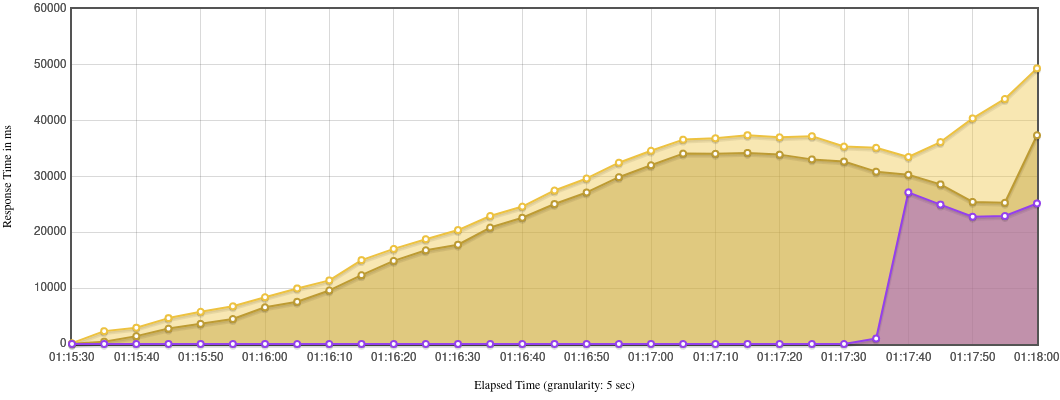
\includegraphics[width=.9\linewidth]{without_nginx_min_max_medianflotResponseTimePercentilesOverTime.png}  
		\caption{A minimum, medián és maximum válaszidők időbeli eloszlása}
		\label{fig:without_nginx_min_median_max_over_time}
	\end{subfigure}
	
	\caption[Helpdesk backend terheléses teszt Nginx nélkül]{Nginx nélkül futó helpdesk backend terheléses teszt eredménye $6~000$ felhasználóval}
	\floatfoot{Forrás: saját ábra}
\end{figure}


Ha ezt a tényt összevetjük azzal, hogy
\begin{itemize}
	\item a különböző tesztesetekre adott válaszidő különbözik (\ref{fig:without_nginx_percentil} ábra),
	\item az esetek 0.19\%-ában \textit{Connection reset} hibát kap a JMeter,
	\item valamint hogy a processzorigény nem tér el az Nginx-el együtt futtatott teszttől,
\end{itemize}
akkor arra a következtetésre juthatunk, hogy az Nginx használata nem hogy rontotta volna a válaszidőt, hanem sokkal inkább kiszámíthatóbbá jobban tervezhetővé tette azt.


\subsection{HikariCP}\label{sec:hikari}
\Aref{fig:10_hikari} ábrán látszódik hogy a HikariCP-ben beállított 10 kapcsolat hamar elfogy, már mérés elején 189-re nő, és tartósan ott is marad a pool-ra várakozók száma.

Ha az adatbázissal való kapcsolat a szűk keresztmetszet, akkor a HikariCP pooljának megnövelésével jelentős javulás lenne elérhető.

Ezért a megismételt a JMeter tesztben a backendben megháromszoroztam a HikariCP pooljának a méretét. A mérési eredmények --\ref{tabl:hikari_30}~táblázat-- nem mutatnak eltérést az első, kiinduló állapothoz képest.

\begin{table}[hbt]
	\begin{tabular}{ccccc|c|cc}
		\multicolumn{5}{c|}{Válaszidő [$ms$]}  & Áteresztőképesség & \multicolumn{2}{c}{Válasz [\%]}	\\
		Átlag & Max. & Medián & P90 & P95 &	[Tranzakció$/s$] & $<3s$& $<6s$ \\
		\hline 
		15 220,66 & 32 136 & 23 836,00 & 28 876 & 29 177 & 278,42 & 12,51 & 26,41 \\
	\end{tabular} 
	\caption{30 adatbázis-kapcsolattal futó helpdesk backend terheléses teszt eredménye $6~000$ felhasználóval}
	\label{tabl:hikari_30}
\end{table}



\begin{figure}[hbt]
	\begin{subfigure}{.49\textwidth}
		\centering
		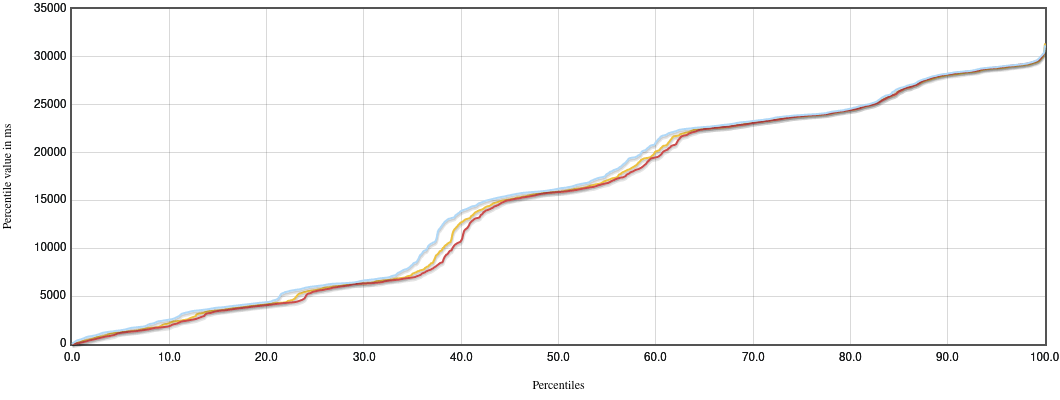
\includegraphics[width=.9\linewidth]{hikari_30_flotResponseTimesPercentiles.png}  
		\caption{A válaszidők percentilis eloszlása}
	\end{subfigure}
	\begin{subfigure}{.49\textwidth}
		\centering
		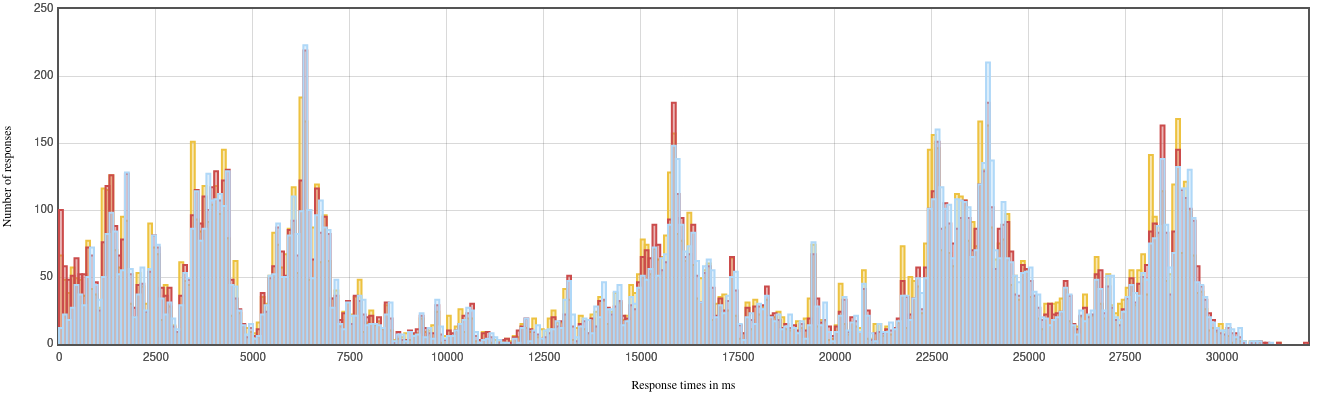
\includegraphics[width=.9\linewidth]{hikari_30_flotResponseTimeDistribution.png}  
		\caption{A válaszidők eloszlása}
	\end{subfigure}
	
	\caption[Helpdesk backend terheléses teszt módosított HikariCp beállításokkal]{30 adatbázis-kapcsolattal futó helpdesk backend terheléses teszt eredménye $6~000$ felhasználóval}
	\floatfoot{Forrás: saját ábra}
\end{figure}


\Aref{fig:hikari_30} ábrán látszódik, hogy mind a harminc pool részt vesz az adatbáziskapcsolatokban. A kapcsolatra várakozók száma 169 lett, csak azzal a 20-szal lett kevesebb, amit hozzáadtunk a poolhoz.


\begin{figure}[hbt] 
	\centering
	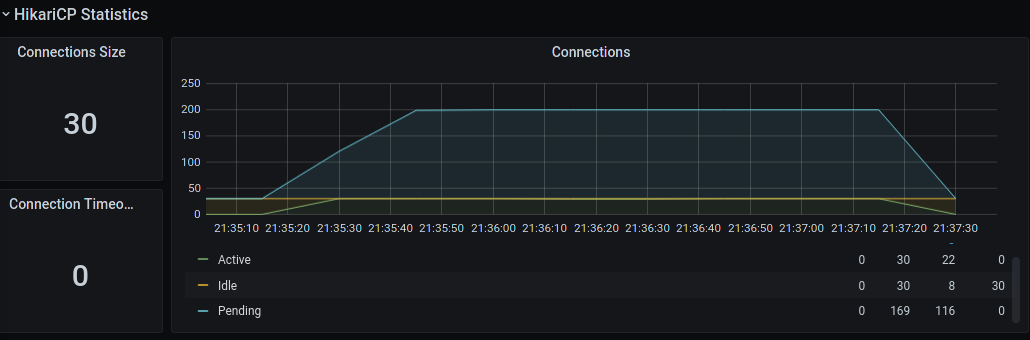
\includegraphics[width=0.8\textwidth]{hikari_30.png}
	\caption{HikariCP adatbázis-kapcsolatai}
	\label{fig:hikari_30}
	\floatfoot{Forrás: saját ábra}
\end{figure}

Mivel a teszteredményekben nincs jelentős változás, nem a HikariCp a szűk keresztmetszet.

\pagebreak
\subsection{Megnövekedett processzorigény}
\Aref{fig:cpu_1_instance} ábrán látszódik hogy még van szabad processzoridő. Ha a helpdesk backend  képes lenne magának még processzoridőt allokálni, azzal javulhatna a rendszer áteresztőképessége. 

Ha a processzoridő a szűk keresztmetszet, akkor új backend példányok indításával, és így újabb erőforrások bevonásával jelentős javulást lehetne elérni.

Ezért a megismételt JMeter tesztben a backendből három példányt indítottam el. Az eredmények így összemérhetőek maradtak \aref{sec:hikari}. ponttal, hiszen összességében ugyanannyi kapcsolat van a backend és az adatbázis között.


\begin{table}[hbt]
	
		\begin{tabular}{ccccc|c|cc}
			\multicolumn{5}{c|}{Válaszidő [$ms$]}  & Áteresztőképesség & \multicolumn{2}{c}{Válasz [\%]}	\\
			Átlag & Max. & Medián & P90 & P95 &	[Tranzakció$/s$] & $<3s$& $<6s$ \\
			\hline 
			5748,49 & 16 577 & 7452,00 & 11 482,00 & 12 011,95 & 755,62 & 22,23 & 49,01 \\
		\end{tabular} 
	
	\caption{Három példányban futó helpdesk backend terheléses teszt eredménye $6~000$ felhasználóval}
	\label{tabl:3_instance}
\end{table}


\Aref{tabl:3_instance} táblázat adatai alapján kijelenthető,
\begin{itemize}
	\item hogy az átlagos válaszidő 6 másodperc alá esett,
	\item az áteresztőképesség megháromszorozódott,
	\item és a három másodpercen belül érkező válaszok aránya is megduplázódott.
\end{itemize}


\Aref{fig:3_instance} ábrán megjelenített mérési eredményeken látszódik hogy a válaszidők szórása nagy mértékben csökkent, a várható bizonytalanság így már sokkal inkább tolerálható.



\begin{figure}[hbt] 
	\centering
	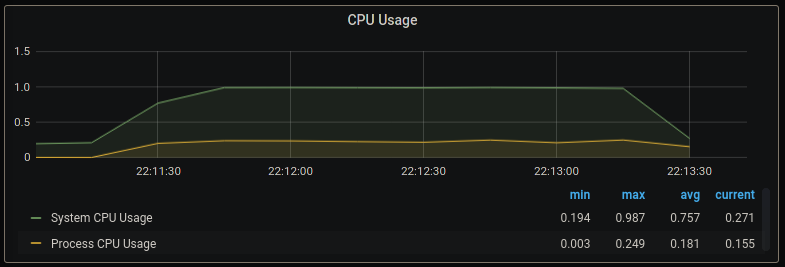
\includegraphics[width=0.6\textwidth]{CPU_3_instance.png}
	\caption{A backend egy példányának a processzor használata}
	\label{fig:3_instance_CPU}
	\floatfoot{Forrás: saját ábra}
\end{figure}



Ha megvizsgáljuk a teszt során mérhető processzor használatot (\ref{fig:3_instance_CPU} ábra), akkor látható, hogy nem maradt már allokálatlan processzoridő. Valószínűleg a két újabb backend példány használta fel a maradék erőforrást.

\begin{figure}[!hbt]
	\begin{subfigure}{.9\textwidth}
		\centering
		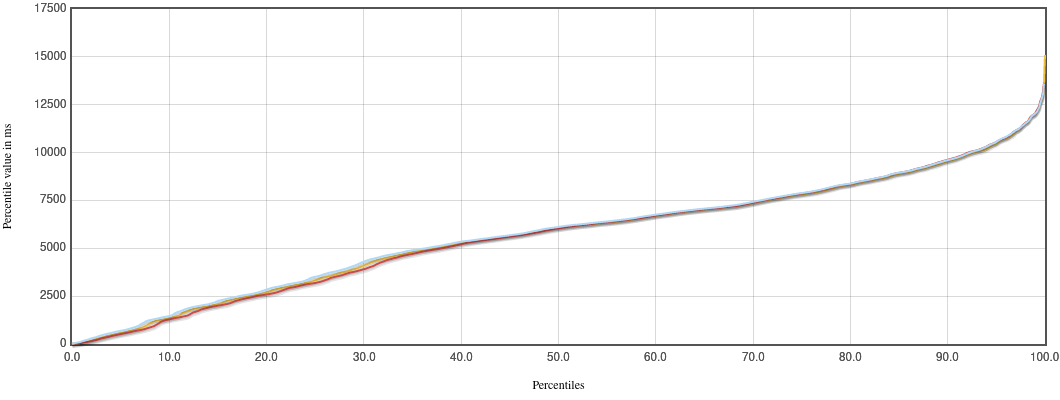
\includegraphics[width=.9\linewidth]{3_instance_flotResponseTimesPercentiles.png}  
		\caption{A válaszidők percentilis eloszlása}
	\end{subfigure}
	\begin{subfigure}{.9\textwidth}
		\centering
		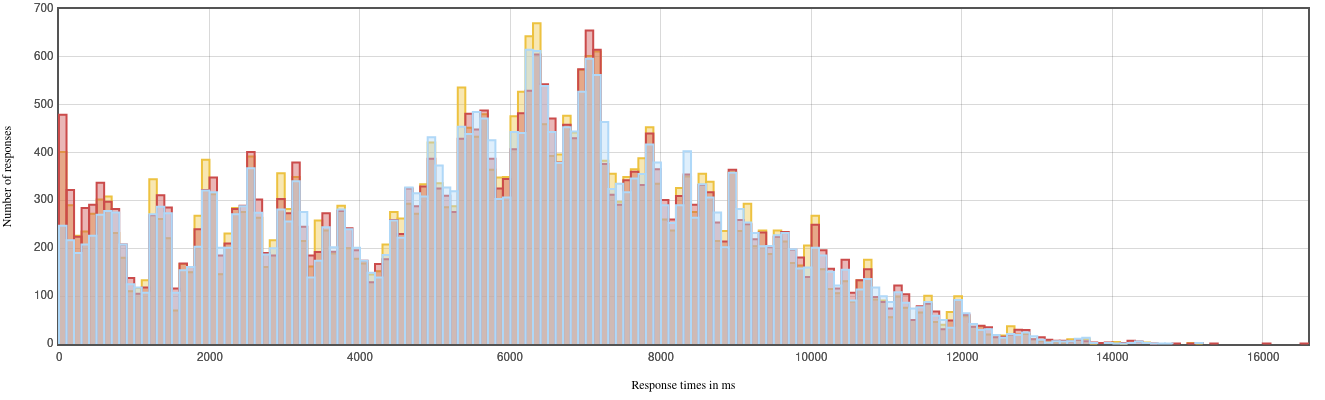
\includegraphics[width=.9\linewidth]{3_instance_flotResponseTimeDistribution.png}  
		\caption{A válaszidők eloszlása}
	\end{subfigure}
	
	\caption[Helpdesk backend terheléses teszt három példánnyal]{Három példányban futó helpdesk backend terheléses teszt eredménye $6~000$ felhasználóval}
	\floatfoot{Forrás: saját ábra}
	\label{fig:3_instance}
\end{figure}



\subsection{Szűk keresztmetszet meghatározása}\label{sec:szuk_keresztmetszet}
A mérések alapján világosan látszik hogy a szűk keresztmetszetet a backend kevés processzorideje jelentette. Újabb példányok indításával jelentősen megnövekedett a rendszer áteresztőképessége, és lecsökkent a válaszideje.

\Aref{fig:3_instance_CPU} ábrán az is látszódik, hogy a futtatásra használt számítógépnek nincs annyi számítási kapacitása, mint amennyire a backendnek szüksége lenne. Így a valódi szűk keresztmetszetet a rendelkezésre álló erőforrások jelentik.


\pagebreak

\section{Összevetés a követelményekkel}
Az elvégzett tesztekből látszódik, hogy horizontális skálázhatósággal jelentősen megnövelhető a helpdesk alkalmazás áteresztőképessége, és csökkenthető a válaszideje.

\subsection{Átlagos teljesítmény vizsgálata}
Az alkalmazás minden probléma nélkül teljesíti az átlagos terhelés esetére meghatározott követelményeket. Legrosszabb esetben is 1 másodpercen belül válaszol.

\subsection{Csúcsteljesítmény vizsgálata}
A rendszerrel szembeni elvárások teljesíthetőségére nem lehet egyértelmű választ adni. A tesztelt számítógépen --erőforráshiány miatt (\ref{sec:szuk_keresztmetszet})-- az alkalmazás nem teljesíti a három másodperces válaszidőre vonatkozó megkötést.

A mérésekből azonban arra lehet következtetni, hogy a valós rendszer --akár több különálló számítógépen-- bírni fogja a terhelést, nem jelent majd gondot neki a csúcsterhelés során sem feladatinak ellátása.



